% Options for packages loaded elsewhere
\PassOptionsToPackage{unicode}{hyperref}
\PassOptionsToPackage{hyphens}{url}
%
\documentclass[
]{article}
\usepackage{amsmath,amssymb}
\usepackage{lmodern}
\usepackage{iftex}
\ifPDFTeX
  \usepackage[T1]{fontenc}
  \usepackage[utf8]{inputenc}
  \usepackage{textcomp} % provide euro and other symbols
\else % if luatex or xetex
  \usepackage{unicode-math}
  \defaultfontfeatures{Scale=MatchLowercase}
  \defaultfontfeatures[\rmfamily]{Ligatures=TeX,Scale=1}
\fi
% Use upquote if available, for straight quotes in verbatim environments
\IfFileExists{upquote.sty}{\usepackage{upquote}}{}
\IfFileExists{microtype.sty}{% use microtype if available
  \usepackage[]{microtype}
  \UseMicrotypeSet[protrusion]{basicmath} % disable protrusion for tt fonts
}{}
\makeatletter
\@ifundefined{KOMAClassName}{% if non-KOMA class
  \IfFileExists{parskip.sty}{%
    \usepackage{parskip}
  }{% else
    \setlength{\parindent}{0pt}
    \setlength{\parskip}{6pt plus 2pt minus 1pt}}
}{% if KOMA class
  \KOMAoptions{parskip=half}}
\makeatother
\usepackage{xcolor}
\IfFileExists{xurl.sty}{\usepackage{xurl}}{} % add URL line breaks if available
\IfFileExists{bookmark.sty}{\usepackage{bookmark}}{\usepackage{hyperref}}
\hypersetup{
  pdftitle={Conceitos Sobre Distribuições de Probabilidade},
  pdfauthor={Gabriel D'assumpção de Carvalho},
  hidelinks,
  pdfcreator={LaTeX via pandoc}}
\urlstyle{same} % disable monospaced font for URLs
\usepackage[margin=1in]{geometry}
\usepackage{color}
\usepackage{fancyvrb}
\newcommand{\VerbBar}{|}
\newcommand{\VERB}{\Verb[commandchars=\\\{\}]}
\DefineVerbatimEnvironment{Highlighting}{Verbatim}{commandchars=\\\{\}}
% Add ',fontsize=\small' for more characters per line
\usepackage{framed}
\definecolor{shadecolor}{RGB}{248,248,248}
\newenvironment{Shaded}{\begin{snugshade}}{\end{snugshade}}
\newcommand{\AlertTok}[1]{\textcolor[rgb]{0.94,0.16,0.16}{#1}}
\newcommand{\AnnotationTok}[1]{\textcolor[rgb]{0.56,0.35,0.01}{\textbf{\textit{#1}}}}
\newcommand{\AttributeTok}[1]{\textcolor[rgb]{0.77,0.63,0.00}{#1}}
\newcommand{\BaseNTok}[1]{\textcolor[rgb]{0.00,0.00,0.81}{#1}}
\newcommand{\BuiltInTok}[1]{#1}
\newcommand{\CharTok}[1]{\textcolor[rgb]{0.31,0.60,0.02}{#1}}
\newcommand{\CommentTok}[1]{\textcolor[rgb]{0.56,0.35,0.01}{\textit{#1}}}
\newcommand{\CommentVarTok}[1]{\textcolor[rgb]{0.56,0.35,0.01}{\textbf{\textit{#1}}}}
\newcommand{\ConstantTok}[1]{\textcolor[rgb]{0.00,0.00,0.00}{#1}}
\newcommand{\ControlFlowTok}[1]{\textcolor[rgb]{0.13,0.29,0.53}{\textbf{#1}}}
\newcommand{\DataTypeTok}[1]{\textcolor[rgb]{0.13,0.29,0.53}{#1}}
\newcommand{\DecValTok}[1]{\textcolor[rgb]{0.00,0.00,0.81}{#1}}
\newcommand{\DocumentationTok}[1]{\textcolor[rgb]{0.56,0.35,0.01}{\textbf{\textit{#1}}}}
\newcommand{\ErrorTok}[1]{\textcolor[rgb]{0.64,0.00,0.00}{\textbf{#1}}}
\newcommand{\ExtensionTok}[1]{#1}
\newcommand{\FloatTok}[1]{\textcolor[rgb]{0.00,0.00,0.81}{#1}}
\newcommand{\FunctionTok}[1]{\textcolor[rgb]{0.00,0.00,0.00}{#1}}
\newcommand{\ImportTok}[1]{#1}
\newcommand{\InformationTok}[1]{\textcolor[rgb]{0.56,0.35,0.01}{\textbf{\textit{#1}}}}
\newcommand{\KeywordTok}[1]{\textcolor[rgb]{0.13,0.29,0.53}{\textbf{#1}}}
\newcommand{\NormalTok}[1]{#1}
\newcommand{\OperatorTok}[1]{\textcolor[rgb]{0.81,0.36,0.00}{\textbf{#1}}}
\newcommand{\OtherTok}[1]{\textcolor[rgb]{0.56,0.35,0.01}{#1}}
\newcommand{\PreprocessorTok}[1]{\textcolor[rgb]{0.56,0.35,0.01}{\textit{#1}}}
\newcommand{\RegionMarkerTok}[1]{#1}
\newcommand{\SpecialCharTok}[1]{\textcolor[rgb]{0.00,0.00,0.00}{#1}}
\newcommand{\SpecialStringTok}[1]{\textcolor[rgb]{0.31,0.60,0.02}{#1}}
\newcommand{\StringTok}[1]{\textcolor[rgb]{0.31,0.60,0.02}{#1}}
\newcommand{\VariableTok}[1]{\textcolor[rgb]{0.00,0.00,0.00}{#1}}
\newcommand{\VerbatimStringTok}[1]{\textcolor[rgb]{0.31,0.60,0.02}{#1}}
\newcommand{\WarningTok}[1]{\textcolor[rgb]{0.56,0.35,0.01}{\textbf{\textit{#1}}}}
\usepackage{longtable,booktabs,array}
\usepackage{calc} % for calculating minipage widths
% Correct order of tables after \paragraph or \subparagraph
\usepackage{etoolbox}
\makeatletter
\patchcmd\longtable{\par}{\if@noskipsec\mbox{}\fi\par}{}{}
\makeatother
% Allow footnotes in longtable head/foot
\IfFileExists{footnotehyper.sty}{\usepackage{footnotehyper}}{\usepackage{footnote}}
\makesavenoteenv{longtable}
\usepackage{graphicx}
\makeatletter
\def\maxwidth{\ifdim\Gin@nat@width>\linewidth\linewidth\else\Gin@nat@width\fi}
\def\maxheight{\ifdim\Gin@nat@height>\textheight\textheight\else\Gin@nat@height\fi}
\makeatother
% Scale images if necessary, so that they will not overflow the page
% margins by default, and it is still possible to overwrite the defaults
% using explicit options in \includegraphics[width, height, ...]{}
\setkeys{Gin}{width=\maxwidth,height=\maxheight,keepaspectratio}
% Set default figure placement to htbp
\makeatletter
\def\fps@figure{htbp}
\makeatother
\setlength{\emergencystretch}{3em} % prevent overfull lines
\providecommand{\tightlist}{%
  \setlength{\itemsep}{0pt}\setlength{\parskip}{0pt}}
\setcounter{secnumdepth}{5}
\usepackage{amsmath}
\usepackage{fancyhdr}
\usepackage{listings}
\usepackage{xcolor}
\usepackage{cancel}
\renewcommand{\CancelColor}{\color{red}}
\usepackage{fvextra}
  \DefineVerbatimEnvironment{Highlighting}{Verbatim}{
    breaksymbolleft={},
    showspaces = false,
    showtabs = false,
    breaklines,
    commandchars=\\\{\}
  }
\pagestyle{fancy}
\fancyhf{}  
\fancyhead[L]{\nouppercase{\leftmark}}
\fancyhead[R]{\thepage}
\fancyfoot[C]{Página \thepage}
\fancyhead[C]{}

\ifLuaTeX
  \usepackage{selnolig}  % disable illegal ligatures
\fi

\title{Conceitos Sobre Distribuições de Probabilidade}
\author{Gabriel D'assumpção de Carvalho}
\date{2025-08-01}

\begin{document}
\maketitle

{
\setcounter{tocdepth}{2}
\tableofcontents
}
\newpage

\hypertarget{introduuxe7uxe3o}{%
\section{Introdução}\label{introduuxe7uxe3o}}

Neste relatório, abordamos os principais conceitos relacionados às seguintes distribuições de probabilidade: Bernoulli, Binomial, Multinomial, Poisson, Exponencial, Geométrica, Hipergeométrica, Gama e Weibull. Essas distribuições são fundamentais para a modelagem estatística, especialmente em contextos de análise de sobrevivência, pois permitem descrever a probabilidade de ocorrência de eventos discretos (como sucesso, falha, etc.) e contínuos (como tempo até a falha ou tempo de vida útil de um sistema).

Neste estudo, geraremos amostras com 1000 observações de cada uma dessas distribuições. Em seguida, construiremos gráficos de barras para variáveis discretas e histogramas para variáveis contínuas, a fim de visualizar o comportamento de suas respectivas probabilidades.

\begin{Shaded}
\begin{Highlighting}[]
\CommentTok{\# Configuração de reprodutibilidade}
\NormalTok{n }\OtherTok{\textless{}{-}} \DecValTok{1000}
\FunctionTok{set.seed}\NormalTok{(}\DecValTok{42}\NormalTok{)}
\end{Highlighting}
\end{Shaded}

\hypertarget{distribuiuxe7uxf5es-discretas}{%
\section{Distribuições Discretas}\label{distribuiuxe7uxf5es-discretas}}

Distribuições discretas descrevem variáveis aleatórias que podem assumir valores finitos ou contáveis. Abaixo, exploramos algumas das distribuições discretas mais utilizadas na prática estatística.

\hypertarget{distribuiuxe7uxe3o-de-bernoulli}{%
\subsection{Distribuição de Bernoulli}\label{distribuiuxe7uxe3o-de-bernoulli}}

A distribuição de Bernoulli é uma das mais importantes distribuições de probabilidade. Qualquer situação que envolva apenas dois desfechos possíveis pode ser modelada como uma variável de Bernoulli. Os dois resultados possíveis são: sucesso (1) ou fracasso (0). A probabilidade de sucesso é denotada por \(p\) e a de fracasso por \(q = 1 - p\).

A função de massa de probabilidade (FMP) da distribuição de Bernoulli é dada por:

\[
P(X = x) = p^x (1 - p)^{1 - x}, \quad x \in \{0, 1\}
\]

Onde \(X\) representa a variável aleatória que indica o resultado do experimento.

\hypertarget{esperanuxe7a}{%
\subsubsection{Esperança}\label{esperanuxe7a}}

A esperança da variável \(X_i\) é dada por:

\[
E(X) = \mathbb{P}(X = 1) \cdot 1 + \mathbb{P}(X = 0) \cdot 0 = p
\]

\hypertarget{variuxe2ncia}{%
\subsubsection{Variância}\label{variuxe2ncia}}

Utilizando a identidade \(\text{Var}(X_i) = E(X_i^2) - [E(X_i)]^2\), temos:

\[
\text{Var}(X) = E(X^2) - [E(X)]^2 = p(1 - p) = pq
\]

Sendo:

\begin{itemize}
  \item $E(X)$: esperança (média) da variável aleatória $X$;
  \item $\text{Var}(X)$: variância de $X$;
  \item $p$: probabilidade de sucesso;
  \item $q$: probabilidade de fracasso.
\end{itemize}

\hypertarget{exemplo-bernoulli}{%
\subsubsection{Exemplo}\label{exemplo-bernoulli}}

\begin{Shaded}
\begin{Highlighting}[]
\NormalTok{p }\OtherTok{\textless{}{-}} \FloatTok{0.7}
\NormalTok{bernoulli }\OtherTok{\textless{}{-}} \FunctionTok{rbinom}\NormalTok{(n, }\DecValTok{1}\NormalTok{, p)}

\FunctionTok{barplot}\NormalTok{(}\FunctionTok{table}\NormalTok{(bernoulli),}
  \AttributeTok{main =} \StringTok{"Distribuição Bernoulli (p = 0.7)"}\NormalTok{,}
  \AttributeTok{names.arg =} \FunctionTok{c}\NormalTok{(}\StringTok{"0"}\NormalTok{, }\StringTok{"1"}\NormalTok{),}
  \AttributeTok{col =} \FunctionTok{c}\NormalTok{(}\StringTok{"\#ff0000"}\NormalTok{, }\StringTok{"\#55a802"}\NormalTok{),}
  \AttributeTok{ylab =} \StringTok{"Frequência"}\NormalTok{,}
  \AttributeTok{xlab =} \StringTok{"Valor"}
\NormalTok{)}
\end{Highlighting}
\end{Shaded}

\begin{figure}

{\centering 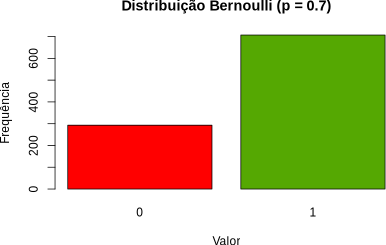
\includegraphics{7_activity_files/figure-latex/bernoulli-plot-1} 

}

\caption{Distribuição de Bernoulli}\label{fig:bernoulli-plot}
\end{figure}

\begin{Shaded}
\begin{Highlighting}[]
\FunctionTok{print}\NormalTok{(}\FunctionTok{paste}\NormalTok{(}\StringTok{"Esperança:"}\NormalTok{, }\FunctionTok{mean}\NormalTok{(bernoulli), }\StringTok{" | "}\NormalTok{, }\StringTok{"p = "}\NormalTok{, p))}
\end{Highlighting}
\end{Shaded}

\begin{verbatim}
## [1] "Esperança: 0.707  |  p =  0.7"
\end{verbatim}

\begin{Shaded}
\begin{Highlighting}[]
\FunctionTok{print}\NormalTok{(}\FunctionTok{paste}\NormalTok{(}\StringTok{"Variância:"}\NormalTok{, }\FunctionTok{round}\NormalTok{(}\FunctionTok{var}\NormalTok{(bernoulli), }\DecValTok{4}\NormalTok{), }\StringTok{" | "}\NormalTok{, }\StringTok{"p * q = "}\NormalTok{, p }\SpecialCharTok{*}\NormalTok{ (}\DecValTok{1} \SpecialCharTok{{-}}\NormalTok{ p)))}
\end{Highlighting}
\end{Shaded}

\begin{verbatim}
## [1] "Variância: 0.2074  |  p * q =  0.21"
\end{verbatim}

Podemos observar que a média e a variância empíricas da amostra seguem de perto os valores teóricos \(E(X) = p\) e \(\text{Var}(X) = pq\), confirmando a adequação da distribuição.

\hypertarget{distribuiuxe7uxe3o-binomial}{%
\subsection{Distribuição Binomial}\label{distribuiuxe7uxe3o-binomial}}

A distribuição binomial generaliza a Bernoulli para \(n\) repetições independentes do mesmo experimento. Cada tentativa tem probabilidade de sucesso \(p\) e fracasso \(q = 1 - p\). A variável aleatória \(X\) representa o número de sucessos em \(n\) tentativas.

A função de massa de probabilidade é dada por:

\[
P(X = k) = \binom{n}{k} p^k (1 - p)^{n - k}, \quad k = 0, 1, \ldots, n
\]

Onde:

\begin{itemize}
  \item $n$: número total de tentativas;
  \item $k$: número de sucessos;
  \item $\binom{n}{k}$: coeficiente binomial, que representa o número de combinações de $n$ termos, $k$ a $k$.
\end{itemize}

Nota-se que quando \(n = 1\), a distribuição binomial se reduz à distribuição de Bernoulli. Por isso, foi utilizado \texttt{rbinom(n,\ 1,\ p)} no exemplo \ref{exemplo-bernoulli}.

\hypertarget{esperanuxe7a-1}{%
\subsubsection{Esperança}\label{esperanuxe7a-1}}

A esperança da variável \(X_i\) é dada por:

\[
E(X^i) = \sum_{k=0}^{n} k^i \cdot \binom{n}{k} p^k \cdot (1 - p)^{n - k}
= \sum_{k=0}^{n} k \cdot k^{i-1} \cdot \binom{n}{k} \cdot p \cdot p^{k-1} \cdot (1 - p)^{n - k}
\]

\[
= \sum_{k=0}^{n} \cancel{k} \cdot k^{i-1} \cdot \frac{n \cdot (n - 1)!}{\cancel{k} \cdot (k - 1)! \cdot (n - k)!} 
\cdot p \cdot p^{k-1} \cdot (1 - p)^{n - k}
= n \cdot p \sum_{k=0}^{n} k^{i-1} \cdot \frac{(n - 1)!}{(k - 1)! \cdot (n - k)!} 
\cdot p^{k-1} \cdot (1 - p)^{n - k}
\]

Aplicando a substituição de índice:

\[
k = j + 1 \Rightarrow k - 1 = j
\]

Obtemos:

\[
E(X^i) = n \cdot p \sum_{j=0}^{n-1} (j + 1)^{i-1} \cdot \frac{(n - 1)!}{j! \cdot (n - j - 1)!} 
\cdot p^{j} \cdot (1 - p)^{n - j - 1}
= n \cdot p \sum_{j=0}^{n-1} (j + 1)^{i-1} \cdot \binom{n - 1}{j} \cdot p^{j} \cdot (1 - p)^{n - j - 1}
\]

Reconhecendo a estrutura esperada de um momento da distribuição binomial de ordem \(n-1\), temos:

\[
E(X^i) = n \cdot p \cdot E\left[(j + 1)^{i-1}\right], \quad \text{onde } j \sim \text{Binomial}(n - 1, p)
\]

Portanto, ao aplicar a propriedade recursiva para o primeiro momento (\(i = 1\)), temos:

\[
E(X) = n \cdot p \cdot E(X^{0}) = n \cdot p \cdot 1 = n \cdot p
\]

\hypertarget{variuxe2ncia-1}{%
\subsubsection{Variância}\label{variuxe2ncia-1}}

Utilizando a identidade \(\text{Var}(X_i) = E(X_i^2) - [E(X_i)]^2\), temos:

\[
\text{Var}(X) = E(X^2) - [E(X)]^2 
= n \cdot p \cdot E[(j + 1)^{2 - 1}] - n^2 \cdot p^2 
= n \cdot p \cdot ((n - 1)\cdot p + 1) - n^2 \cdot p^2
\]

\[
= n \cdot p \cdot (n \cdot p - p + 1) - n^2 \cdot p^2 
= \cancel{n^2 \cdot p^2} - n \cdot p^2 + n \cdot p - \cancel{n^2 \cdot p^2} 
= n \cdot p \cdot (1 - p) = n \cdot p \cdot q
\]

\hypertarget{exemplo-binomial}{%
\subsubsection{Exemplo}\label{exemplo-binomial}}

\begin{Shaded}
\begin{Highlighting}[]
\NormalTok{k }\OtherTok{\textless{}{-}} \DecValTok{100}

\NormalTok{binomial }\OtherTok{\textless{}{-}} \FunctionTok{rbinom}\NormalTok{(n, k, }\FloatTok{0.7}\NormalTok{)}

\FunctionTok{barplot}\NormalTok{(}
  \FunctionTok{table}\NormalTok{(binomial),}
  \AttributeTok{main =} \StringTok{"Distribuição Binomial (n = 1000, k = 100, p = 0.7)"}\NormalTok{,}
  \AttributeTok{col =} \StringTok{"\#55a802"}\NormalTok{,}
  \AttributeTok{ylab =} \StringTok{"Frequência"}\NormalTok{,}
  \AttributeTok{xlab =} \StringTok{"Número de Sucessos"}
\NormalTok{)}
\end{Highlighting}
\end{Shaded}

\begin{figure}

{\centering 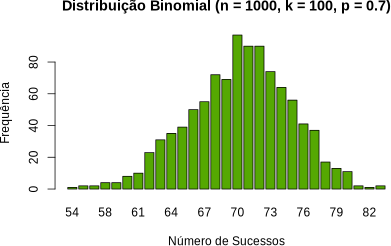
\includegraphics{7_activity_files/figure-latex/binomial-plot-1} 

}

\caption{Distribuição Binomial}\label{fig:binomial-plot}
\end{figure}

\begin{Shaded}
\begin{Highlighting}[]
\FunctionTok{print}\NormalTok{(}\FunctionTok{paste}\NormalTok{(}\StringTok{"Esperança:"}\NormalTok{, }\FunctionTok{mean}\NormalTok{(binomial), }\StringTok{" | "}\NormalTok{, }\StringTok{"k * p = "}\NormalTok{, k }\SpecialCharTok{*}\NormalTok{ p))}
\end{Highlighting}
\end{Shaded}

\begin{verbatim}
## [1] "Esperança: 70.24  |  k * p =  70"
\end{verbatim}

\begin{Shaded}
\begin{Highlighting}[]
\FunctionTok{print}\NormalTok{(}\FunctionTok{paste}\NormalTok{(}\StringTok{"Variância:"}\NormalTok{, }\FunctionTok{round}\NormalTok{(}\FunctionTok{var}\NormalTok{(binomial), }\DecValTok{4}\NormalTok{), }\StringTok{" | "}\NormalTok{, }\StringTok{"k * p * q = "}\NormalTok{, k }\SpecialCharTok{*}\NormalTok{ p }\SpecialCharTok{*}\NormalTok{ (}\DecValTok{1} \SpecialCharTok{{-}}\NormalTok{ p)))}
\end{Highlighting}
\end{Shaded}

\begin{verbatim}
## [1] "Variância: 21.2917  |  k * p * q =  21"
\end{verbatim}

Com isso, podemos ver que a média e a variância empírica da amostra de uma variável aleatória que segue uma distribuição binomial com parâmetros \(n\) e \(p\) se aproximam dos valores teóricos \(E(X) = n \cdot p\) e \(\text{Var}(X) = n \cdot p \cdot q\), confirmando as propiedades demonstradas.

\hypertarget{distribuiuxe7uxe3o-multinomial}{%
\subsection{Distribuição Multinomial}\label{distribuiuxe7uxe3o-multinomial}}

A distribuição multinomial é uma generalização da distribuição binomial para experimentos com mais de dois possíveis resultados. Ela é usada quando realizamos \(n\) experimentos independentes, cada um resultando em exatamente uma das \(k\) categorias possíveis. Cada categoria \(i = 1, 2, \ldots, k\) tem uma probabilidade associada \(p_i\), com \(\sum_{i=1}^{k} p_i = 1\). A função de massa de probabilidade da distribuição é dada por:

\[
P(X_1 = n_1, \ldots, X_k = n_k) = \binom{n}{n_1, n_2, \ldots, n_k} \cdot p_1^{n_1} \cdots p_k^{n_k}
\]

Podemos expandir o coeficiente multinomial como:

\[
= \frac{n!}{n_1! \cdot \cancel{(n - n_1)!}} \cdot \frac{\cancel{(n - n_1)!}}{n_2! \cdot \cancel{(n - n_1 - n_2)!}} \cdots \frac{\cancel{(n - n_1 - \cdots - n_{k-1})!}}{n_k! \cdot 0!}
\cdot p_1^{n_1} \cdots p_k^{n_k}
\]

Resultando em:

\[
= \frac{n!}{n_1! \cdots n_k!} \cdot p_1^{n_1} \cdots p_k^{n_k}
\]

Onde:

\begin{itemize}
  \item $X_i$: número de ocorrências da categoria $i$;
  \item $n$: número total de experimentos;
  \item $n_i$: número de vezes que a categoria $i$ ocorreu (ou seja, $X_i = n_i$);
  \item $p_i$: probabilidade de ocorrência da categoria $i$.
\end{itemize}

\hypertarget{esperanuxe7a-2}{%
\subsubsection{Esperança}\label{esperanuxe7a-2}}

A esperança da variável \(X_i\) é dada por:

\[
E(X_i) = \sum_{x_1 + \cdots + x_k = n} X_i \cdot \frac{n!}{x_1! \cdots x_k!} \cdot p_1^{x_1} \cdots p_k^{x_k}
\]

Aplicando a manipulação:

\[
E(X_i) = n \cdot p_i \cdot 
\cancelto{1}{
  \sum \frac{(n - 1)!}{
    (x_1 - \delta_{1i})! \cdots (x_k - \delta_{ki})!
  }
  \cdot p_1^{x_1 - \delta_{1i}} \cdots p_k^{x_k - \delta_{ki}}
}
\text{,} \quad 
\delta_{ji} =
\begin{cases}
  1, & \text{se } j = i \\
  0, & \text{caso contrário}
\end{cases}
\]

Essa soma corresponde a uma distribuição multinomial de ordem \((n - 1)\) e soma 1:

\[
\Rightarrow E(X_i) = n \cdot p_i
\]

\hypertarget{variuxe2ncia-2}{%
\subsubsection{Variância}\label{variuxe2ncia-2}}

Utilizando a identidade \(\text{Var}(X_i) = E(X_i^2) - [E(X_i)]^2\), temos:

\[
E(X_i^2) = E(X_i(X_i - 1)) + E(X_i)
\]

Sabendo que:

\[
E(X_i(X_i - 1)) = n(n - 1)p_i^2 \quad \text{e} \quad E(X_i) = np_i
\]

Substituímos:

\[
\text{Var}(X_i) = n(n - 1)p_i^2 + np_i - (np_i)^2
= n^2p_i^2 - np_i^2 + np_i - n^2p_i^2
\]

\[
= -np_i^2 + np_i = np_i(1 - p_i)
\]

Logo, a variância da variável \(X_i\) na distribuição multinomial é:

\[
\text{Var}(X_i) = np_i(1 - p_i)
\]

\hypertarget{exemplo-multinomial}{%
\subsubsection{Exemplo}\label{exemplo-multinomial}}

\begin{Shaded}
\begin{Highlighting}[]
\NormalTok{class }\OtherTok{\textless{}{-}} \DecValTok{4}
\NormalTok{ps }\OtherTok{\textless{}{-}} \FunctionTok{c}\NormalTok{(p, }\FunctionTok{rep}\NormalTok{((}\DecValTok{1} \SpecialCharTok{{-}}\NormalTok{ p) }\SpecialCharTok{/}\NormalTok{ (class }\SpecialCharTok{{-}} \DecValTok{1}\NormalTok{), class }\SpecialCharTok{{-}} \DecValTok{1}\NormalTok{))}
\NormalTok{multnom }\OtherTok{\textless{}{-}} \FunctionTok{rmultinom}\NormalTok{(n, }\AttributeTok{size =}\NormalTok{ k, }\AttributeTok{prob =}\NormalTok{ ps)}
\NormalTok{frequencias }\OtherTok{\textless{}{-}} \FunctionTok{rowSums}\NormalTok{(multnom)}
\end{Highlighting}
\end{Shaded}

\newpage

\begin{Shaded}
\begin{Highlighting}[]
\FunctionTok{barplot}\NormalTok{(}
\NormalTok{  frequencias,}
  \AttributeTok{names.arg =} \FunctionTok{paste}\NormalTok{(}\StringTok{"Classe"}\NormalTok{, }\DecValTok{1}\SpecialCharTok{:}\NormalTok{class),}
  \AttributeTok{col =} \FunctionTok{colorRampPalette}\NormalTok{(}\FunctionTok{c}\NormalTok{(}\StringTok{"\#b2df8a"}\NormalTok{, }\StringTok{"\#33a02c"}\NormalTok{))(class),}
  \AttributeTok{main =} \FunctionTok{paste}\NormalTok{(}\StringTok{"Distribuição Multinomial: n ="}\NormalTok{, n, }\StringTok{", size ="}\NormalTok{, k, }\StringTok{"class ="}\NormalTok{, class),}
  \AttributeTok{cex.main =} \FloatTok{0.9}\NormalTok{,}
  \AttributeTok{xlab =} \StringTok{"Classe"}\NormalTok{,}
  \AttributeTok{ylab =} \StringTok{"Frequência"}
\NormalTok{)}
\end{Highlighting}
\end{Shaded}

\begin{figure}

{\centering 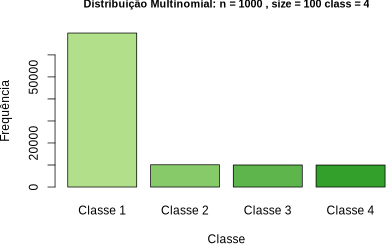
\includegraphics{7_activity_files/figure-latex/multinom-plot-1} 

}

\caption{Distribuição Multinomial}\label{fig:multinom-plot}
\end{figure}

\begin{Shaded}
\begin{Highlighting}[]
\NormalTok{E\_empirica }\OtherTok{\textless{}{-}} \FunctionTok{rowSums}\NormalTok{(multnom) }\SpecialCharTok{/}\NormalTok{ n}
\NormalTok{E\_teorica }\OtherTok{\textless{}{-}}\NormalTok{ k }\SpecialCharTok{*}\NormalTok{ ps}

\FunctionTok{data.frame}\NormalTok{(}
  \AttributeTok{Classe =} \FunctionTok{paste0}\NormalTok{(}\StringTok{"Classe "}\NormalTok{, }\DecValTok{1}\SpecialCharTok{:}\FunctionTok{length}\NormalTok{(ps)),}
  \StringTok{\textasciigrave{}}\AttributeTok{E(empírica}\StringTok{\textasciigrave{}} \OtherTok{=} \FunctionTok{round}\NormalTok{(E\_empirica, }\DecValTok{3}\NormalTok{),}
  \StringTok{\textasciigrave{}}\AttributeTok{E(teórica}\StringTok{\textasciigrave{}} \OtherTok{=} \FunctionTok{round}\NormalTok{(E\_teorica, }\DecValTok{3}\NormalTok{)}
\NormalTok{)}
\end{Highlighting}
\end{Shaded}

\begin{verbatim}
##     Classe E.empírica E.teórica
## 1 Classe 1     69.929        70
## 2 Classe 2     10.101        10
## 3 Classe 3      9.999        10
## 4 Classe 4      9.971        10
\end{verbatim}

Dado um experimento multinomial com \(n = 1000\), tamanho de ensaio \(k = 100\), probabilidade da primeira classe \(p_1 = 0.7\) e as probabilidades restantes definidas como \(p_i = \frac{1 - p_1}{\text{número de classes} - 1}\), totalizando 6 classes, observa-se que a média empírica se aproxima da média teórica, confirmando assim as propriedades esperadas da distribuição multinomial.

\hypertarget{distribuiuxe7uxe3o-de-poisson}{%
\subsection{Distribuição de Poisson}\label{distribuiuxe7uxe3o-de-poisson}}

A distribuição de poisson é uma distribuição discreta que modela o número de eventos que ocorrem em um intervalo fixo de tempo, tendo uma taxa média de ocorrência \(lambda\), constante e independente do tempo. Com isso, a função de massa de probabilidade é dada por:

\[
P(X = k) = \frac{\lambda^k \cdot e^{-\lambda}}{k!}, \quad k = 0, 1, 2, \ldots
\]

Onde:

\begin{itemize}
  \item $k$: Valor que a variável aleatória $X$ pode assumir (número de eventos);
  \item $\lambda$: Taxa média de ocorrência de eventos no intervalo considerado;
  \item $e$: Base do logaritmo natural, aproximadamente 2.71828.
\end{itemize}

\hypertarget{esperanuxe7a-3}{%
\subsubsection{Esperança}\label{esperanuxe7a-3}}

A esperança da variável \(X\) é dada por:

\[
E(X) = \sum_{k=0}^{\infty} k \cdot P(X = k) = \sum_{k=0}^{\infty} k \cdot \frac{\lambda^k \cdot e^{-\lambda}}{k!}
\]

\[
= \sum_{k=1}^{\infty} \lambda \cdot \cancel{k} \cdot \frac{\lambda^{k-1} \cdot e^{-\lambda}}{\cancel{k} \cdot (k-1)!} = \lambda \cdot e^{-\lambda} \sum_{k=1}^{\infty} \frac{\lambda^{k-1}}{(k-1)!}
\]

\[
= \lambda \cdot e^{-\lambda} \cdot \cancelto{e^\lambda}{\left[\frac{\lambda^0}{0!} + \frac{\lambda^1}{1!} + \frac{\lambda^2}{2!} + \ldots \right]} = \lambda
\]

\hypertarget{variuxe2ncia-3}{%
\subsubsection{Variância}\label{variuxe2ncia-3}}

A variância da variável que segue a distribuição de Poisson é dada por:

\[
\text{Var}(X) = E(X^2) - [E(X)]^2 = \sum_{k=0}^{\infty} k^2 \cdot P(X = k) - \lambda^2 
\]

\[ 
E(X^2)= 1^2\left[\frac{e^{-\lambda} \cdot \lambda^1}{1!}\right] + 2^2\left[\frac{e^{-\lambda} \cdot \lambda^2}{2!}\right] + 3^2\left[\frac{e^{-\lambda} \cdot \lambda^3}{3!}\right] + \ldots +  n^2\left[\frac{e^{-\lambda} \cdot \lambda^n}{n!} \right] + \cdots
\]

\[
= e^{-\lambda} \cdot \lambda \left[1 + 2\cdot\lambda + 3\cdot\frac{\lambda^2}{2!} + \ldots + n\cdot\frac{\lambda^{n-1}}{(n-1)!} + \cdots \right]
\]

\[
= e^{-\lambda} \cdot \lambda \cdot \sum_{n=1}^{\infty} n \cdot \frac{\lambda^{n-1}}{(n-1)!}\text{, onde } n - 1 = k \text{ e } n = k + 1 
\]

\[
= e^{-\lambda} \cdot \lambda \cdot \left[
0 + \frac{\lambda}{1!} + \frac{\cancel{2}\cdot \lambda^2}{\cancel{2!}} + \frac{\cancel{3}\cdot \lambda^{3}}{\cancel{3}\cdot 2!} + \ldots + e^{\lambda}
\right]
\]

\[
= e^{-\lambda} \cdot \lambda \cdot \left[
\lambda \cancelto{e^{\lambda}}{\left(1 + \frac{\lambda}{1!} + \frac{\lambda^2}{2!} + \cdots + \frac{\lambda^{k-1}}{(k-1)!}\right)} + e^{\lambda}
\right] = e^{-\lambda} \cdot \lambda \cdot [\lambda \cdot e^{\lambda} + e^{\lambda}] = e^{0} \cdot \lambda^2 + e^{0} \cdot \lambda = \lambda^2 + \lambda
\]

\[
\text{Var}(X) = \cancel{\lambda^2} + \lambda - \cancel{\lambda^2} = \lambda
\]

\hypertarget{exemplo-poisson}{%
\subsubsection{Exemplo}\label{exemplo-poisson}}

\begin{Shaded}
\begin{Highlighting}[]
\NormalTok{lambda }\OtherTok{\textless{}{-}} \DecValTok{5}
\NormalTok{poisson }\OtherTok{\textless{}{-}} \FunctionTok{rpois}\NormalTok{(n, lambda)}

\FunctionTok{barplot}\NormalTok{(}
  \FunctionTok{table}\NormalTok{(poisson),}
  \AttributeTok{main =} \FunctionTok{paste}\NormalTok{(}\StringTok{"Distribuição de Poisson (lambda ="}\NormalTok{, lambda, }\StringTok{")"}\NormalTok{),}
  \AttributeTok{col =} \StringTok{"\#55a802"}\NormalTok{,}
  \AttributeTok{ylab =} \StringTok{"Frequência"}\NormalTok{,}
  \AttributeTok{xlab =} \StringTok{"Número de Eventos"}
\NormalTok{)}
\end{Highlighting}
\end{Shaded}

\begin{figure}

{\centering 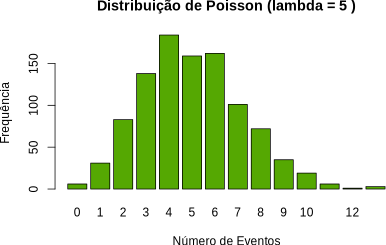
\includegraphics{7_activity_files/figure-latex/poisson-plot-1} 

}

\caption{Distribuição de Poisson}\label{fig:poisson-plot}
\end{figure}

\begin{Shaded}
\begin{Highlighting}[]
\FunctionTok{print}\NormalTok{(}\FunctionTok{paste}\NormalTok{(}\StringTok{"Esperança:"}\NormalTok{, }\FunctionTok{mean}\NormalTok{(poisson), }\StringTok{" | "}\NormalTok{, }\StringTok{"lambda = "}\NormalTok{, lambda))}
\end{Highlighting}
\end{Shaded}

\begin{verbatim}
## [1] "Esperança: 5.019  |  lambda =  5"
\end{verbatim}

\begin{Shaded}
\begin{Highlighting}[]
\FunctionTok{print}\NormalTok{(}\FunctionTok{paste}\NormalTok{(}\StringTok{"Variância:"}\NormalTok{, }\FunctionTok{round}\NormalTok{(}\FunctionTok{var}\NormalTok{(poisson), }\DecValTok{4}\NormalTok{), }\StringTok{" | "}\NormalTok{, }\StringTok{"lambda = "}\NormalTok{, lambda))}
\end{Highlighting}
\end{Shaded}

\begin{verbatim}
## [1] "Variância: 4.8395  |  lambda =  5"
\end{verbatim}

Portanto, podemos observar que a média e a variância empírica da amostra de uma variável aleatória que segue uma distribuição de Poisson com parâmetro \(\lambda\) se aproximam dos valores teóricos \(E(X) = \lambda\) e \(\text{Var}(X) = \lambda\), confirmando as propriedades esperadas da distribuição.

\hypertarget{distribuiuxe7uxe3o-geomuxe9trica}{%
\subsection{Distribuição Geométrica}\label{distribuiuxe7uxe3o-geomuxe9trica}}

A distribuição geométrica modela o número de tentativas até a ocorrência do primeiro sucesso em uma sequência de experimentos de Bernoulli independentes. Sua função de massa de probabilidade é dada por:

\[
P(X = k) = (1 - p)^{k - 1} \cdot p, \quad k = 1, 2, \ldots
\]

\hypertarget{esperanuxe7a-4}{%
\subsubsection{Esperança}\label{esperanuxe7a-4}}

A esperança da variável aleatória \(X\) é calculada como:

\[
E(X) = \sum_{k=1}^{\infty} k \cdot P(X = k) = \sum_{k=1}^{\infty} k \cdot (1 - p)^{k - 1} \cdot p = p \cdot \sum_{k=1}^{\infty} k \cdot (1 - p)^{k-1}
\]

Denotando \(q = 1 - p\), reconhecemos que a soma é uma série geométrica diferenciada, cuja soma é:

\[
\sum_{k=1}^{\infty} k \cdot q^{k - 1} = \frac{1}{(1 - q)^2}
\]

Como \(1 - q = p\), temos:

\[
E(X) = \cancel{p} \cdot \frac{1}{p^{\cancel{2}}} = \frac{1}{p}
\]

\hypertarget{variuxe2ncia-4}{%
\subsubsection{Variância}\label{variuxe2ncia-4}}

A variância é obtida por:

\[
\text{Var}(X) = E(X^2) - [E(X)]^2 = E[X(X-1)] + E(X) - \left(\frac{1}{p}\right)^2
\]

onde:

\[
E[X(X-1)] = \sum_{k=2}^{\infty} k(k-1) \cdot q^{k - 1} \cdot p
\]

Utilizando as propriedades das séries geométricas diferenciadas, temos:

\begin{enumerate}
\def\labelenumi{\arabic{enumi}.}
\tightlist
\item
  Primeira derivada:
\end{enumerate}

\[
\sum_{k=1}^{\infty} k \cdot q^{k - 1} = \frac{d}{dq} \sum_{k=0}^{\infty} q^k = \frac{1}{(1 - q)^2}
\]

\begin{enumerate}
\def\labelenumi{\arabic{enumi}.}
\setcounter{enumi}{1}
\tightlist
\item
  Segunda derivada:
\end{enumerate}

\[
\sum_{k=2}^{\infty} k(k-1) \cdot q^{k - 2} = \frac{d^2}{dq^2} \sum_{k=0}^{\infty} q^k = \frac{d^2}{dq^2} \left(\frac{1}{1 - q}\right) = \frac{2}{(1 - q)^3}
\]

Multiplicando por \(q\), obtemos:

\[
\sum_{k=2}^{\infty} k(k-1) \cdot q^{k - 1} = \frac{2q}{(1 - q)^3}
\]

Assim, substituindo na fórmula da variância:

\[
\text{Var}(X) = p \cdot \frac{2q}{(1 - q)^3} + \frac{1}{p} - \frac{1}{p^2} = \frac{2q p}{p^3} + \frac{1}{p} - \frac{1}{p^2} = \frac{2q}{p^2} + \frac{1}{p} - \frac{1}{p^2}
\]

Simplificando os termos:

\[
\text{Var}(X) = \frac{2q + p - 1}{p^2} = \frac{1 - p}{p^2} = \frac{q}{p^2}
\]

\hypertarget{exemplo-geom}{%
\subsubsection{Exemplo}\label{exemplo-geom}}

\begin{Shaded}
\begin{Highlighting}[]
\NormalTok{geom }\OtherTok{\textless{}{-}} \FunctionTok{rgeom}\NormalTok{(n, p) }\SpecialCharTok{+} \DecValTok{1}

\FunctionTok{barplot}\NormalTok{(}
  \FunctionTok{table}\NormalTok{(geom),}
  \AttributeTok{main =} \FunctionTok{paste}\NormalTok{(}\StringTok{"Distribuição Geométrica (p ="}\NormalTok{, p, }\StringTok{")"}\NormalTok{),}
  \AttributeTok{col =} \StringTok{"\#55a802"}\NormalTok{,}
  \AttributeTok{ylab =} \StringTok{"Frequência"}\NormalTok{,}
  \AttributeTok{xlab =} \StringTok{"Número de Tentativas"}
\NormalTok{)}
\end{Highlighting}
\end{Shaded}

\begin{figure}

{\centering 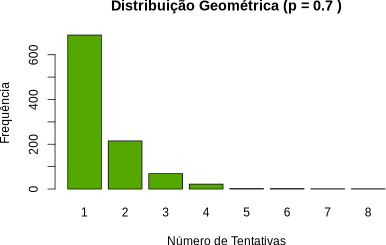
\includegraphics{7_activity_files/figure-latex/geom-plot-1} 

}

\caption{Distribuição Geométrica}\label{fig:geom-plot}
\end{figure}
\newpage

\begin{Shaded}
\begin{Highlighting}[]
\FunctionTok{print}\NormalTok{(}\FunctionTok{paste}\NormalTok{(}\StringTok{"Esperança:"}\NormalTok{, }\FunctionTok{mean}\NormalTok{(geom), }\StringTok{" | "}\NormalTok{, }\StringTok{"1 / p = "}\NormalTok{, }\FunctionTok{round}\NormalTok{(}\DecValTok{1} \SpecialCharTok{/}\NormalTok{ p, }\DecValTok{4}\NormalTok{)))}
\end{Highlighting}
\end{Shaded}

\begin{verbatim}
## [1] "Esperança: 1.45  |  1 / p =  1.4286"
\end{verbatim}

\begin{Shaded}
\begin{Highlighting}[]
\FunctionTok{print}\NormalTok{(}\FunctionTok{paste}\NormalTok{(}\StringTok{"Variância:"}\NormalTok{, }\FunctionTok{round}\NormalTok{(}\FunctionTok{var}\NormalTok{(geom), }\DecValTok{4}\NormalTok{), }\StringTok{" | "}\NormalTok{, }\StringTok{"q / p\^{}2 = "}\NormalTok{, }\FunctionTok{round}\NormalTok{((}\DecValTok{1} \SpecialCharTok{{-}}\NormalTok{ p) }\SpecialCharTok{/}\NormalTok{ p}\SpecialCharTok{\^{}}\DecValTok{2}\NormalTok{, }\DecValTok{4}\NormalTok{)))}
\end{Highlighting}
\end{Shaded}

\begin{verbatim}
## [1] "Variância: 0.6542  |  q / p^2 =  0.6122"
\end{verbatim}

Como podemos ver o experimento do número de tentativas até o primeiro sucesso, seguindo uma distribuição geométrica com parâmetro \(p\), resulta em uma média e variância empíricas que se aproximam dos valores teóricos \(E(X) = \frac{1}{p}\) e \(\text{Var}(X) = \frac{1 - p}{p^2}\), confirmando as propriedades esperadas da distribuição.

\hypertarget{distribuiuxe7uxe3o-hipergeomuxe9trica}{%
\subsection{Distribuição Hipergeométrica}\label{distribuiuxe7uxe3o-hipergeomuxe9trica}}

\hypertarget{esperanuxe7a-5}{%
\subsubsection{Esperança}\label{esperanuxe7a-5}}

\hypertarget{variuxe2ncia-5}{%
\subsubsection{Variância}\label{variuxe2ncia-5}}

\hypertarget{exemplo-hgeom}{%
\subsubsection{Exemplo}\label{exemplo-hgeom}}

\hypertarget{distribuiuxe7uxf5es-contuxednuas}{%
\section{Distribuições Contínuas}\label{distribuiuxe7uxf5es-contuxednuas}}

Ao contrário das distribuições discretas, as distribuições contínuas modelam variáveis aleatórias que podem assumir um número infinito de valores dentro de um determinado intervalo. Essa característica fundamental implica o uso de cálculo integral para determinar a probabilidade de uma variável aleatória se encontrar em um intervalo específico. A seguir, exploraremos algumas das distribuições contínuas mais proeminentes e amplamente aplicadas no campo da estatística.
Como a variável aleatória \(X\) pode assumir qualquer valor não negativo, a probabilidade de \(X\) assumir um valor específico é zero. Em vez disso, a distribuições contínuas são caracterizadas por uma função de densidade de probabilidade (FDP), que descreve a probabilidade de \(X\) cair dentro de um intervalo específico. A integral da FDP sobre um intervalo fornece a probabilidade de \(X\) estar dentro desse intervalo.

\hypertarget{distribuiuxe7uxe3o-exponencial}{%
\subsection{Distribuição Exponencial}\label{distribuiuxe7uxe3o-exponencial}}

A distribuição exponencial é uma distribuição contínua que modela o tempo entre (distâncias) eventos em um processo de Poisson. Tendo os eventos independentes e ocorrendo a uma taxa constante, a função de densidade de probabilidade (FDP) é dada por:

\[
f(x; \lambda) = \lambda e^{-\lambda x}, \quad x \geq 0
\]

Com isso, a função de distribuição acumulada (FDA) é:
\[
F(x; \lambda) = \mathbb{P}(X \leq x) = 1 - e^{-\lambda x}, \quad x \geq 0
\]

\hypertarget{esperanuxe7a-6}{%
\subsubsection{Esperança}\label{esperanuxe7a-6}}

A esperança da variável \(X\) é dada por:
\[
E(X) = \int_0^\infty x f(x; \lambda) dx
= \int_0^\infty x \lambda e^{-\lambda x} dx = \frac{1}{\lambda}
\]

\hypertarget{variuxe2ncia-6}{%
\subsubsection{Variância}\label{variuxe2ncia-6}}

\[
\text{Var}(X) = E(X^2) - [E(X)]^2 = \int_0^\infty x^2 f(x; \lambda) dx - \left(\frac{1}{\lambda}\right)^2 = \frac{1}{\lambda^2}
\]

\hypertarget{exemplo-exp}{%
\subsubsection{Exemplo}\label{exemplo-exp}}

\begin{Shaded}
\begin{Highlighting}[]
\NormalTok{lambda }\OtherTok{\textless{}{-}} \FloatTok{0.5}
\NormalTok{exp\_data }\OtherTok{\textless{}{-}} \FunctionTok{rexp}\NormalTok{(n, lambda)}
\FunctionTok{hist}\NormalTok{(exp\_data,}
  \AttributeTok{breaks =} \DecValTok{30}\NormalTok{, }\AttributeTok{probability =} \ConstantTok{TRUE}\NormalTok{,}
  \AttributeTok{main =} \FunctionTok{paste}\NormalTok{(}\StringTok{"Distribuição Exponencial (lambda ="}\NormalTok{, lambda, }\StringTok{")"}\NormalTok{),}
  \AttributeTok{xlab =} \StringTok{"Valor"}\NormalTok{, }\AttributeTok{ylab =} \StringTok{"Densidade"}\NormalTok{,}
  \AttributeTok{col =} \StringTok{"\#55a802"}\NormalTok{, }\AttributeTok{border =} \StringTok{"white"}
\NormalTok{)}
\FunctionTok{curve}\NormalTok{(}\FunctionTok{dexp}\NormalTok{(x, lambda), }\AttributeTok{add =} \ConstantTok{TRUE}\NormalTok{, }\AttributeTok{col =} \StringTok{"blue"}\NormalTok{, }\AttributeTok{lwd =} \DecValTok{2}\NormalTok{)}
\FunctionTok{legend}\NormalTok{(}\StringTok{"topright"}\NormalTok{, }\AttributeTok{legend =} \StringTok{"FDP"}\NormalTok{, }\AttributeTok{col =} \StringTok{"blue"}\NormalTok{, }\AttributeTok{lty =} \DecValTok{1}\NormalTok{, }\AttributeTok{lwd =} \DecValTok{2}\NormalTok{)}
\end{Highlighting}
\end{Shaded}

\begin{figure}

{\centering 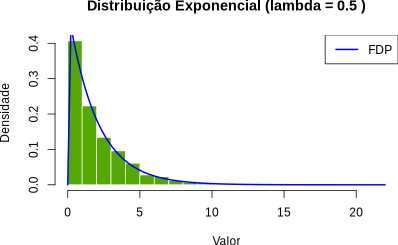
\includegraphics{7_activity_files/figure-latex/exp-plot-1} 

}

\caption{Distribuição Exponencial}\label{fig:exp-plot}
\end{figure}

\begin{Shaded}
\begin{Highlighting}[]
\FunctionTok{print}\NormalTok{(}\FunctionTok{paste}\NormalTok{(}\StringTok{"Esperança:"}\NormalTok{, }\FunctionTok{round}\NormalTok{(}\FunctionTok{mean}\NormalTok{(exp\_data), }\DecValTok{4}\NormalTok{), }\StringTok{" | "}\NormalTok{, }\StringTok{"1 / lambda = "}\NormalTok{, }\FunctionTok{round}\NormalTok{(}\DecValTok{1} \SpecialCharTok{/}\NormalTok{ lambda, }\DecValTok{4}\NormalTok{)))}
\end{Highlighting}
\end{Shaded}

\begin{verbatim}
## [1] "Esperança: 1.9853  |  1 / lambda =  2"
\end{verbatim}

\begin{Shaded}
\begin{Highlighting}[]
\FunctionTok{print}\NormalTok{(}\FunctionTok{paste}\NormalTok{(}\StringTok{"Variância:"}\NormalTok{, }\FunctionTok{round}\NormalTok{(}\FunctionTok{var}\NormalTok{(exp\_data), }\DecValTok{4}\NormalTok{), }\StringTok{" | "}\NormalTok{, }\StringTok{"1 / lambda\^{}2 = "}\NormalTok{, }\FunctionTok{round}\NormalTok{(}\DecValTok{1} \SpecialCharTok{/}\NormalTok{ lambda}\SpecialCharTok{\^{}}\DecValTok{2}\NormalTok{, }\DecValTok{4}\NormalTok{)))}
\end{Highlighting}
\end{Shaded}

\begin{verbatim}
## [1] "Variância: 4.0407  |  1 / lambda^2 =  4"
\end{verbatim}

Como pode ser visto a média e a variância empíricas da amostra de uma variável aleatória que segue uma distribuição exponencial com parâmetro \(\lambda\) se aproximam dos valores teóricos \(E(X) = \frac{1}{\lambda}\) e \(\text{Var}(X) = \frac{1}{\lambda^2}\), confirmando as propriedades esperadas da distribuição.

\hypertarget{distribuiuxe7uxe3o-gamma}{%
\subsection{Distribuição Gamma}\label{distribuiuxe7uxe3o-gamma}}

A distribuição Gamma é uma generalização da distribuição Exponencial, utilizada para modelar o \textbf{tempo até a ocorrência do \(\alpha\)-ésimo evento} em um processo de Poisson. A função densidade de probabilidade (FDP), na parametrização com taxa \(\beta\), é:

\[
f(x; \alpha, \beta) = \frac{\beta^\alpha x^{\alpha - 1} e^{-\beta x}}{\Gamma(\alpha)}, \quad x \geq 0
\]

Quando \(\alpha = 1\), essa expressão se reduz à distribuição Exponencial com parâmetro \(\beta\):

\[
f(x; 1, \beta) = \beta e^{-\beta x}
\]

A função de distribuição acumulada (FDA) é dada pela função gama incompleta regularizada:

\[
F(x; \alpha, \beta) = \int_0^x f(t; \alpha, \beta) dt = \frac{\gamma(\alpha, \beta x)}{\Gamma(\alpha)}
\]

\hypertarget{esperanuxe7a-7}{%
\subsubsection{Esperança}\label{esperanuxe7a-7}}

A esperança da variável aleatória \(X\) é:

\[
\mathbb{E}(X) = \frac{\alpha}{\beta}
\]

\hypertarget{variuxe2ncia-7}{%
\subsubsection{Variância}\label{variuxe2ncia-7}}

A variância é:

\[
\text{Var}(X) = \frac{\alpha}{\beta^2}
\]

\hypertarget{exemplo-gamma}{%
\subsubsection{Exemplo}\label{exemplo-gamma}}

\begin{Shaded}
\begin{Highlighting}[]
\NormalTok{alpha }\OtherTok{\textless{}{-}} \DecValTok{2}
\NormalTok{beta }\OtherTok{\textless{}{-}} \DecValTok{1}
\NormalTok{gamma\_data }\OtherTok{\textless{}{-}} \FunctionTok{rgamma}\NormalTok{(n, }\AttributeTok{shape =}\NormalTok{ alpha, }\AttributeTok{scale =} \DecValTok{1} \SpecialCharTok{/}\NormalTok{ beta)}
\FunctionTok{hist}\NormalTok{(gamma\_data,}
  \AttributeTok{breaks =} \DecValTok{30}\NormalTok{, }\AttributeTok{probability =} \ConstantTok{TRUE}\NormalTok{,}
  \AttributeTok{main =} \FunctionTok{paste}\NormalTok{(}\StringTok{"Distribuição Gamma (alpha ="}\NormalTok{, alpha, }\StringTok{", beta ="}\NormalTok{, beta, }\StringTok{")"}\NormalTok{),}
  \AttributeTok{xlab =} \StringTok{"Valor"}\NormalTok{, }\AttributeTok{ylab =} \StringTok{"Densidade"}\NormalTok{,}
  \AttributeTok{col =} \StringTok{"\#55a802"}\NormalTok{, }\AttributeTok{border =} \StringTok{"white"}
\NormalTok{)}
\FunctionTok{curve}\NormalTok{(}\FunctionTok{dgamma}\NormalTok{(x, }\AttributeTok{shape =}\NormalTok{ alpha, }\AttributeTok{scale =} \DecValTok{1} \SpecialCharTok{/}\NormalTok{ beta), }\AttributeTok{add =} \ConstantTok{TRUE}\NormalTok{, }\AttributeTok{col =} \StringTok{"blue"}\NormalTok{, }\AttributeTok{lwd =} \DecValTok{2}\NormalTok{)}
\FunctionTok{legend}\NormalTok{(}\StringTok{"topright"}\NormalTok{, }\AttributeTok{legend =} \StringTok{"FDP"}\NormalTok{, }\AttributeTok{col =} \StringTok{"blue"}\NormalTok{, }\AttributeTok{lty =} \DecValTok{1}\NormalTok{, }\AttributeTok{lwd =} \DecValTok{2}\NormalTok{)}
\end{Highlighting}
\end{Shaded}

\begin{figure}

{\centering 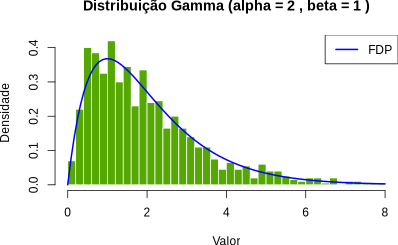
\includegraphics{7_activity_files/figure-latex/gamma-plot-1} 

}

\caption{Distribuição Gamma}\label{fig:gamma-plot}
\end{figure}

\begin{Shaded}
\begin{Highlighting}[]
\FunctionTok{print}\NormalTok{(}\FunctionTok{paste}\NormalTok{(}\StringTok{"Esperança:"}\NormalTok{, }\FunctionTok{round}\NormalTok{(}\FunctionTok{mean}\NormalTok{(gamma\_data), }\DecValTok{4}\NormalTok{), }\StringTok{" | "}\NormalTok{, }\StringTok{"alpha / beta = "}\NormalTok{, }\FunctionTok{round}\NormalTok{(alpha }\SpecialCharTok{/}\NormalTok{ beta, }\DecValTok{4}\NormalTok{)))}
\end{Highlighting}
\end{Shaded}

\begin{verbatim}
## [1] "Esperança: 1.9626  |  alpha / beta =  2"
\end{verbatim}

\begin{Shaded}
\begin{Highlighting}[]
\FunctionTok{print}\NormalTok{(}\FunctionTok{paste}\NormalTok{(}\StringTok{"Variância:"}\NormalTok{, }\FunctionTok{round}\NormalTok{(}\FunctionTok{var}\NormalTok{(gamma\_data), }\DecValTok{4}\NormalTok{), }\StringTok{" | "}\NormalTok{, }\StringTok{"alpha / beta\^{}2 = "}\NormalTok{, }\FunctionTok{round}\NormalTok{(alpha }\SpecialCharTok{/}\NormalTok{ beta}\SpecialCharTok{\^{}}\DecValTok{2}\NormalTok{, }\DecValTok{4}\NormalTok{)))}
\end{Highlighting}
\end{Shaded}

\begin{verbatim}
## [1] "Variância: 1.991  |  alpha / beta^2 =  2"
\end{verbatim}

Podemos observar que a média e a variância empíricas da amostra de uma variável aleatória que segue uma distribuição Gamma com parâmetros \(\alpha\) e \(\beta\) se aproximam dos valores teóricos \(E(X) = \frac{\alpha}{\beta}\) e \(\text{Var}(X) = \frac{\alpha}{\beta^2}\), confirmando as propriedades esperadas da distribuição.

\end{document}
